\chapter{Эксперименты}

\section{Кросс валидация}
Так как в нашем распоряжении было не много размеченных данных, для исключения
переобучения использовалась кросс валидация. Как было описано ранее, предметным
специалистом были предоставлены примерно одинаковые по продолжительности записи
с разных экспериментов, в связи с чем было логично сделать разбиение на группы
именно по ним. Таким образом, всего у нас получилось 8 групп --- по 1 на
валидацию и тестирование и по 6 на обучение. Всего производилось 8
экспериментов (по одному на уникальную тестовую группу). Валидационная группа
выбиралась случайным образом. Метрики замерялись после обучения на тестовой
группе. В качестве финальной метрики бралось среднее от всех экспериментов.

\section{Подсчет метрик}

После получения предсказания встает вопрос о подсчете метрик, ведь при прямом
сравнении, метки с предсказания и с разметки могут быть смещены относительно
друг друга, например, на несколько сэмплов. С учетом пожеланий предметного
специалиста, для исследований которого предоставлялось разметка, было решено
считать истинно положительной активацию, которая была предсказана с точностью
до 5 сэмплов. Таким образом алгоритм подсчета выглядел следующим образом:

Для подсчета TP и FP производилась итерация по активациям предсказания. В
окрестности в 5 сэмплов от каждой метки производился поиск наличия таковой в
исходной разметке. В случае положительного результата предсказание считалось
как TP, иначе --- FP. Для подсчета FN итерация происходила по активациям исходной
разметке, а поиск --- по предсказанию. Активация считалась FN в случае
отсутствия результатов поиска в окрестности истинной метки. Наглядно это
изображено на рис. \ref{fig:metrics} (желтым выделен сигнал, по меткам которого
происходит итерация).

\begin{figure}[!htb]
	\centering
	\subfigure[]{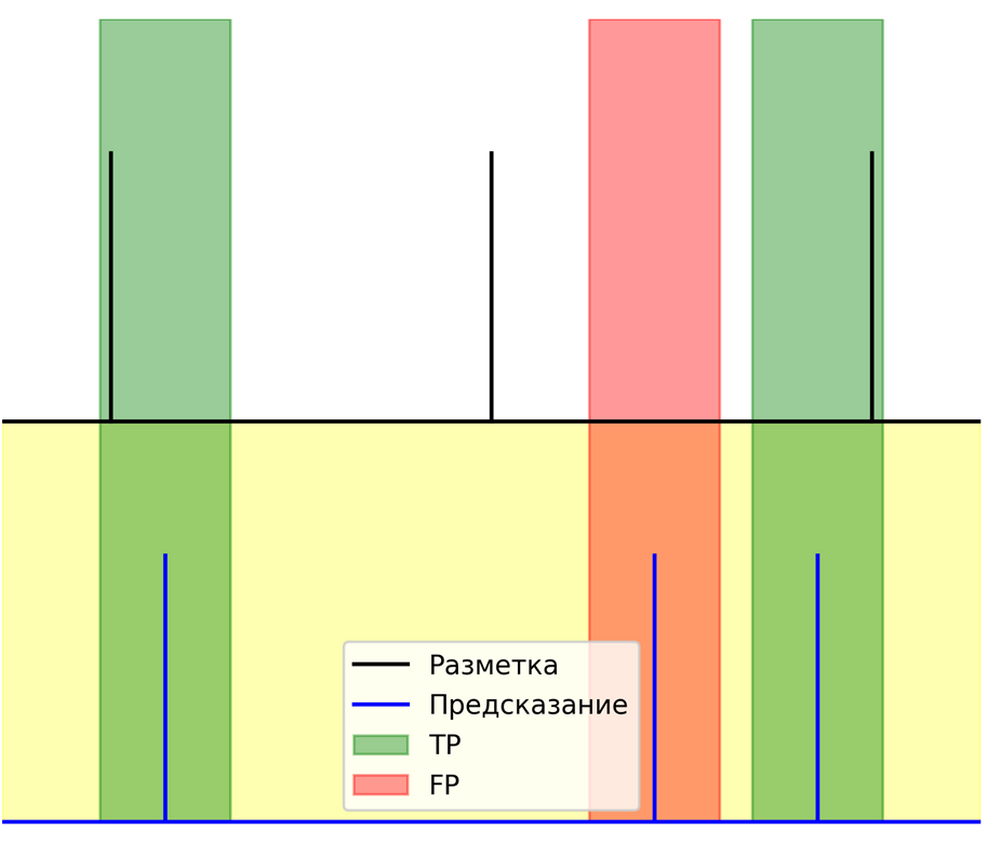
\includegraphics[width=.49\textwidth]{metrics1.png}}
	\subfigure[]{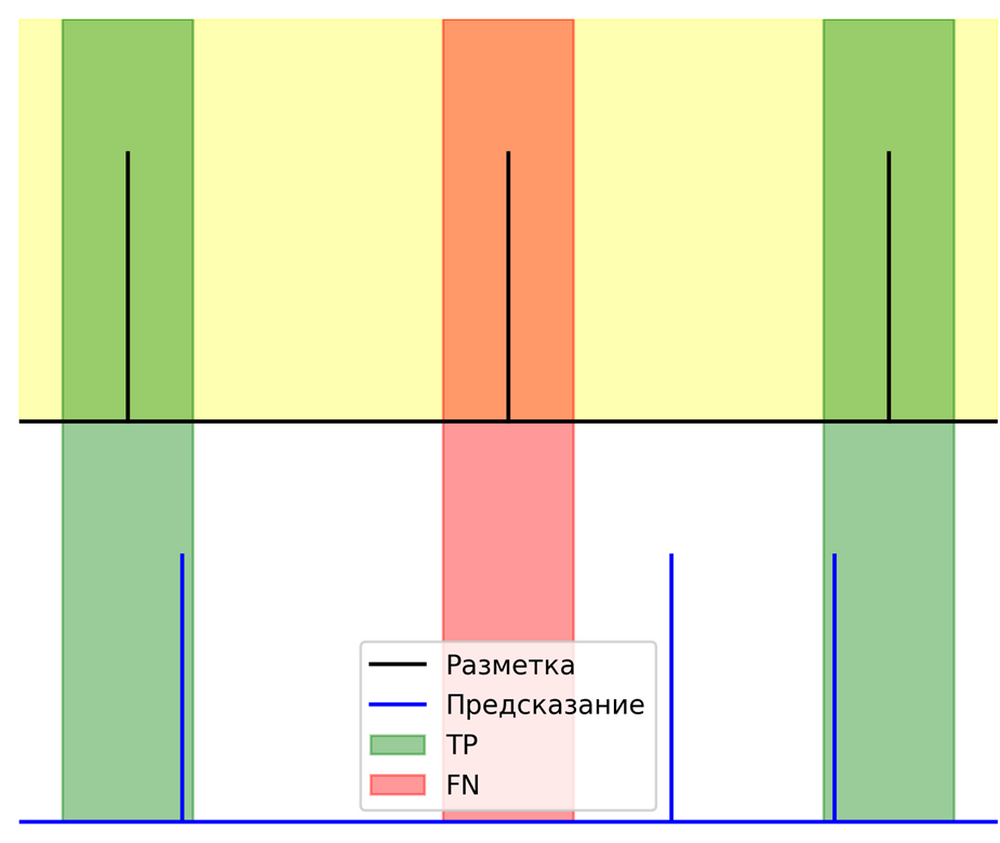
\includegraphics[width=.49\textwidth]{metrics2.png}}
	\caption{(a) Подсчет TP и FP (b) Подсчет FN}
	\label{fig:metrics}
\end{figure}

После подсчета TP, FP и FN по формулам, описанным выше, вычисляется $F_1score$.

\section{Результаты}

В определенный момент времени возникла потребность в ручной проверке и
корректировке истинной разметки. Таким образом, у нас появилась более
качественная разметка, на основе которой были измерены метрики. По сути,
таблицы \ref{tab:results} и \ref{tab:original} сравнивают результаты работы
двух программ: той, которая описана в данной работе, и той, с помощью которой
был выполнен первоначальный анализ. Для более наглядного сопоставления приведен
график итоговой метрики $F_1score$ на рис. \ref{fig:f1score-vs}.

Как показывает сравнение, удалось достичь повышения качества работы на 10\%,
причем данный подход отличается от оригинальной программы тем, что полностью
автоматизирован и не требует тонкой настройки специалистом.

\begin{table}[!htb]
	\centering
	\caption{Результаты экспериментов}
	\label{tab:results}
	\begin{tabular}{@{}cccc@{}}
		\toprule
		\textbf{Эксперимент} & \textbf{Precision} & \textbf{Recall} & \textbf{F1-score} \\ \midrule
		22ph0                & 0.98978            & 0.98777         & 0.98877           \\
		22ph1                & 0.71065            & 0.92843         & 0.80507           \\
		23ph0                & 0.97593            & 0.96674         & 0.97131           \\
		23ph1                & 0.84946            & 0.63552         & 0.72708           \\
		25ph0                & 0.75438            & 0.99047         & 0.85645           \\
		25ph1                & 0.77875            & 0.93807         & 0.85102           \\
		26ph0                & 0.83584            & 0.96802         & 0.89709           \\
		26ph1                & 0.58380            & 0.87136         & 0.69917           \\ \midrule
		\textbf{Среднее}     & 0.81700            & 0.90254         & 0.84638           \\ \bottomrule
	\end{tabular}
\end{table}

\begin{table}[!htb]
	\centering
	\caption{Оригинальная разметка}
	\label{tab:original}
	\begin{tabular}{@{}cccc@{}}
		\toprule
		\textbf{Эксперимент} & \textbf{Precision} & \textbf{Recall} & \textbf{F1-score} \\ \midrule
		22ph0                & 0.98837            & 0.98445         & 0.98641           \\
		22ph1                & 0.98296            & 0.45197         & 0.61922           \\
		23ph0                & 0.97825            & 0.88805         & 0.93097           \\
		23ph1                & 0.96247            & 0.38016         & 0.54504           \\
		25ph0                & 0.96412            & 0.84612         & 0.90128           \\
		25ph1                & 0.37485            & 0.85144         & 0.52054           \\
		26ph0                & 0.99379            & 0.70904         & 0.82761           \\
		26ph1                & 0.98798            & 0.38471         & 0.55378           \\ \midrule
		Среднее              & 0.91848            & 0.69786         & 0.73339           \\ \bottomrule
	\end{tabular}
\end{table}

\begin{figure}[!htb]
	\centering
	\caption{Сравнение $F_1score$ оригинальной разметки и предсказанной}
	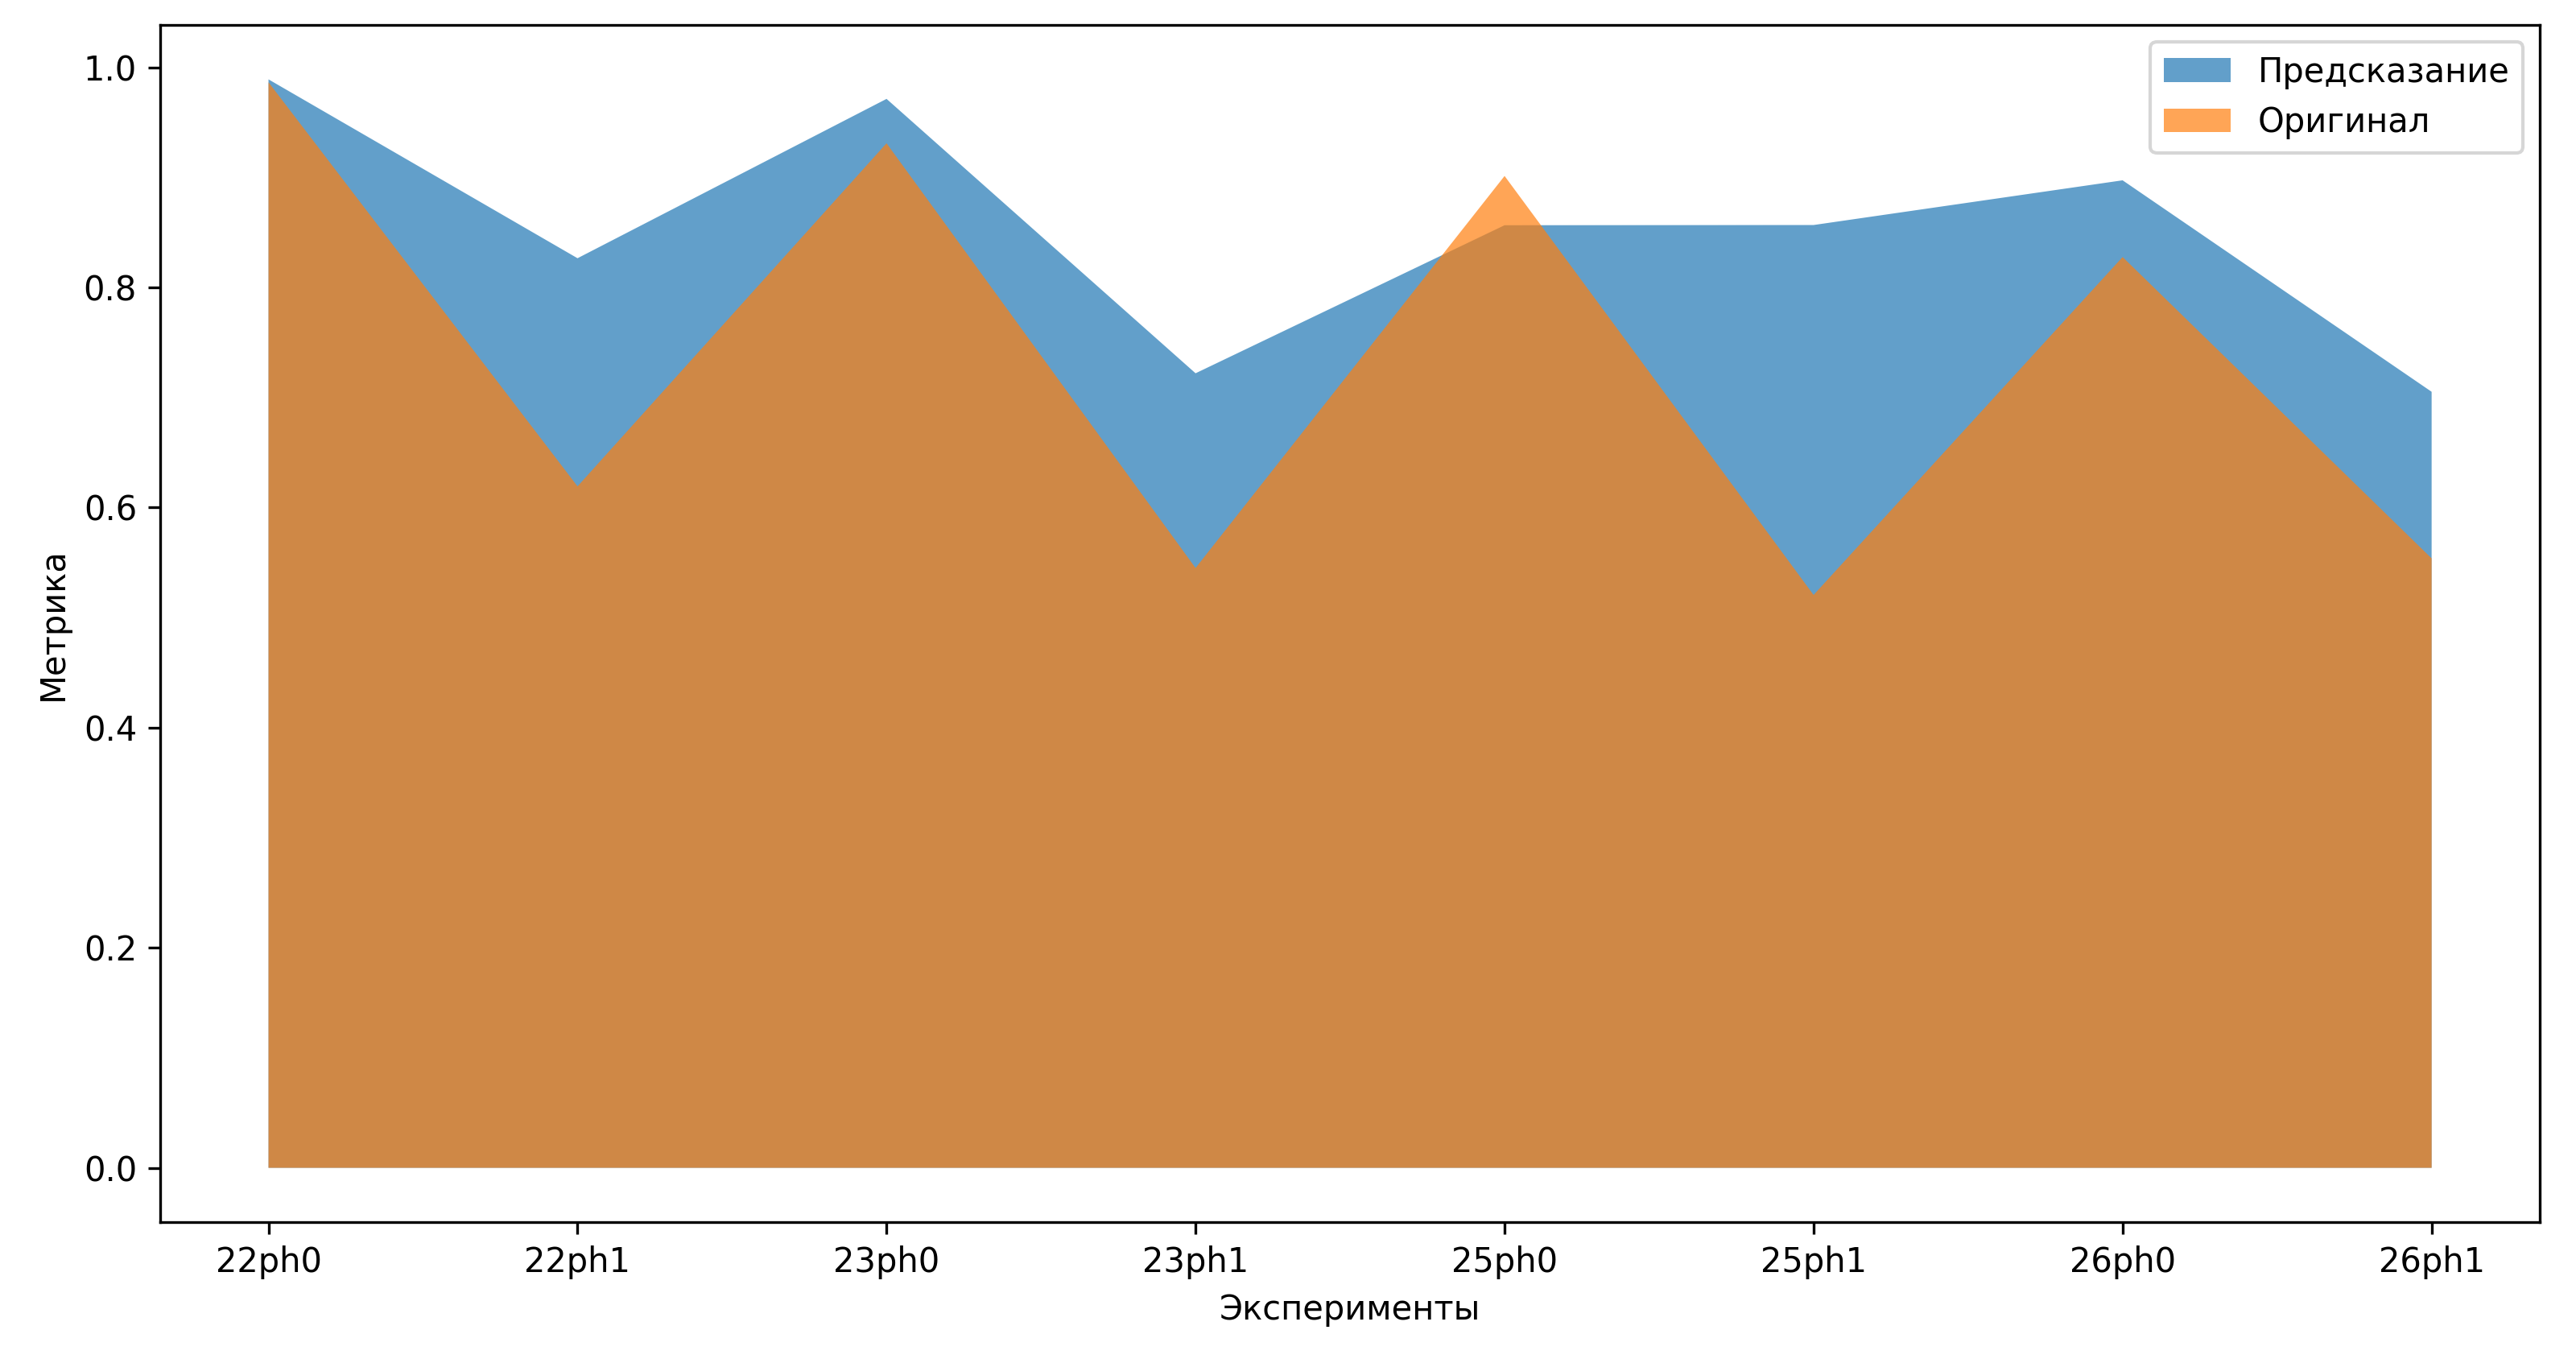
\includegraphics[width=\textwidth]{f1score-cropped.png}
	\label{fig:f1score-vs}
\end{figure}
